\indent Para corroborar la performance de nuestro algoritmo, trabajamos con distintos tipos de grafos.\\

Como la complejidad calculada fue O( E * V * LOG(V)) decidimos fijar E y tener V movil.\\
Trabajando con grafos circulares variando el tamaño de entrada entre 0 y 10000 y corriendo la misma medición varias veces sacamos un promedio del mismo para obtener datos  más relevantes y obtuvimos el siguiente resultado:

\vspace*{0.3cm} \vspace*{0.3cm}
  \begin{center}
 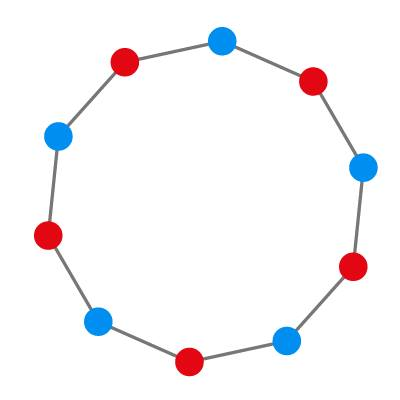
\includegraphics[scale=0.5]{./ej3/circular.jpg}
 	{\\Gráfico 3.4.1 - Grafo circular}
  \end{center}
  \vspace*{0.3cm}
  
  \vspace*{0.3cm} \vspace*{0.3cm}
  \begin{center}
 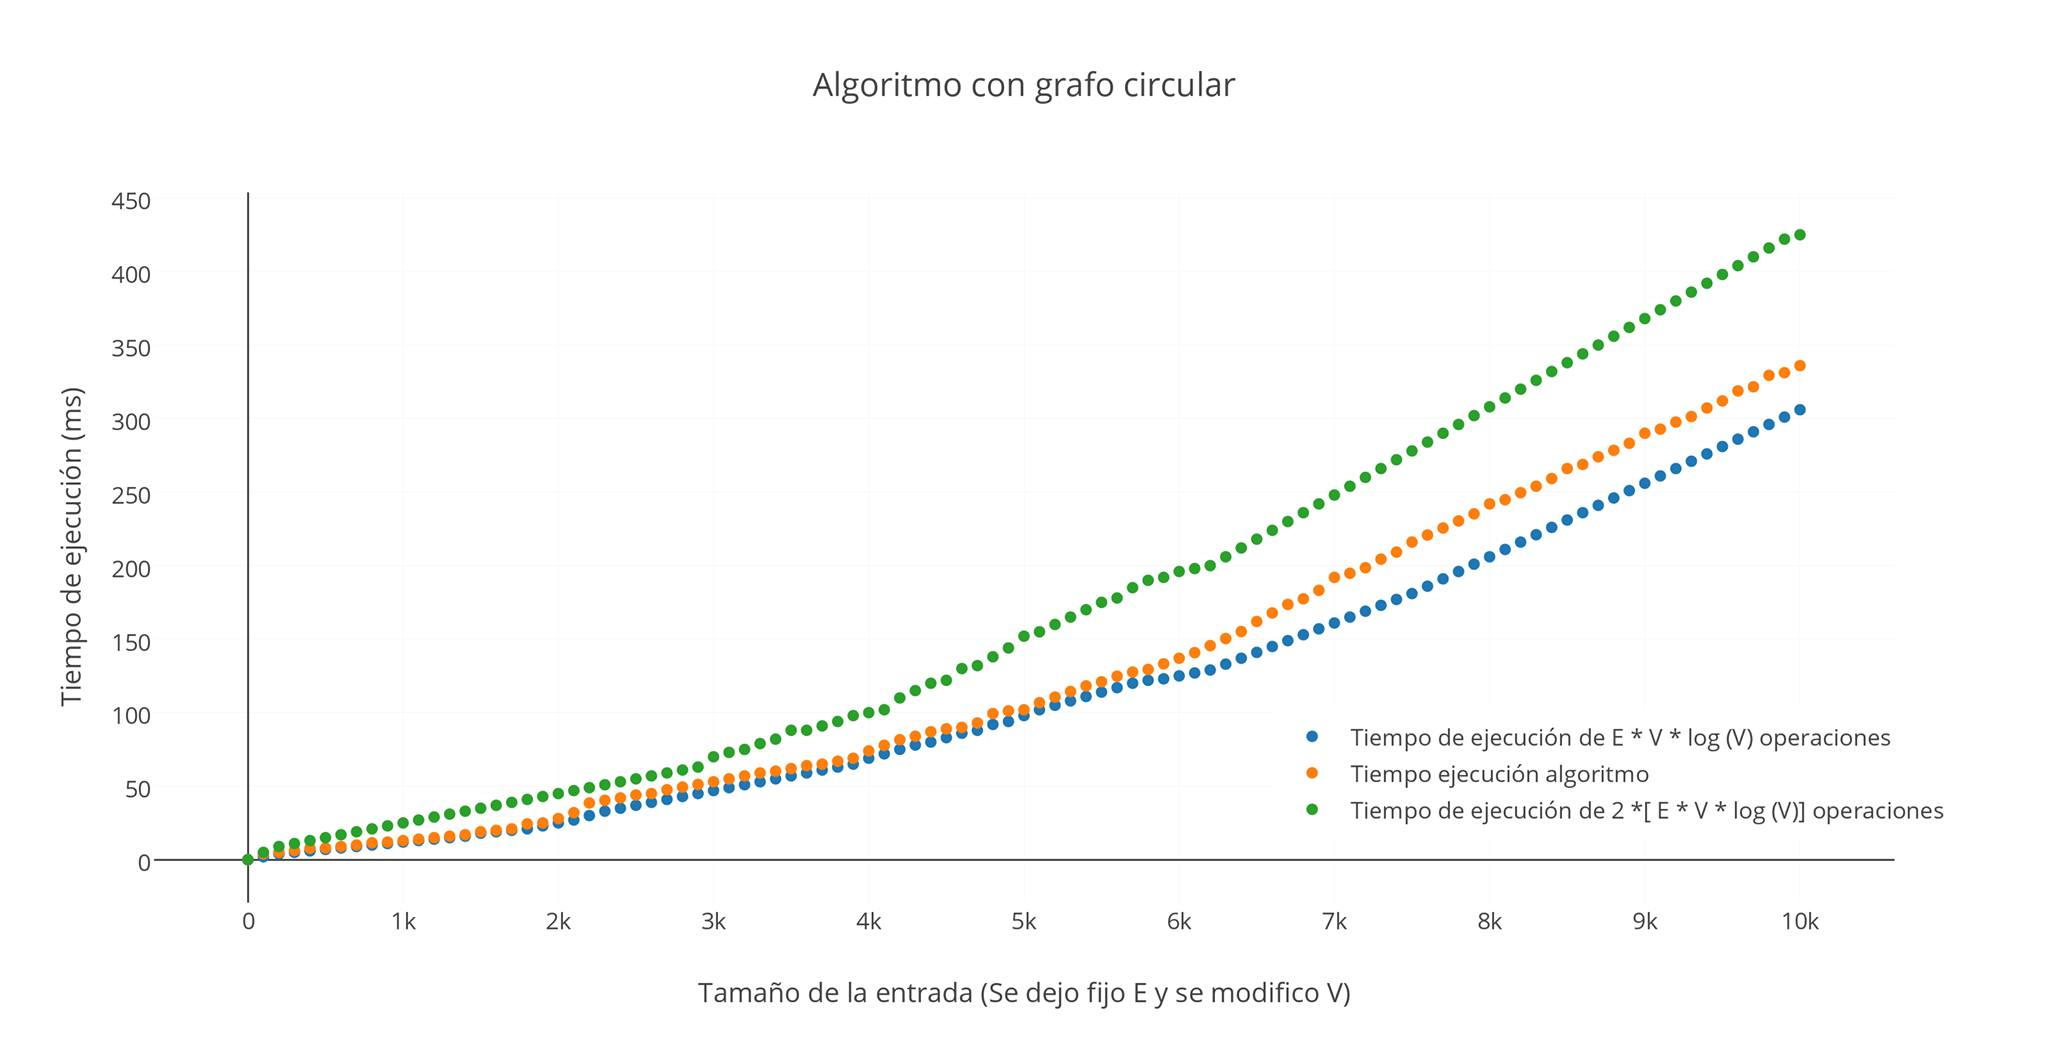
\includegraphics[scale=0.28]{./ej3/circular2.jpg}
 	{Gráfico 3.4.2 - Medición grafo circular}
  \end{center}
  \vspace*{0.3cm}


En la figura 3.4.1 se puede observar el tipo de grafo que utilizamos. En la figura 3.4.2, se puede ver como el tiempo de ejecución de nuestro algoritmo se encuentra entre los tiempos de realizar E * LOG(V) operaciones y 2*[E * LOG(V)] demostrando como en este 
tipo de grafo la complejidad calculada de nuestro algoritmo fue correcta.\\




Trabajando con grafos completos variando el tamaño de entrada entre 0 y 10000 y realizando la misma medición varias veces sacamos un promedio del mismo para obtener datos más consistentes y obtuvimos el siguiente resultado:

\vspace*{0.3cm} \vspace*{0.3cm}
  \begin{center}
 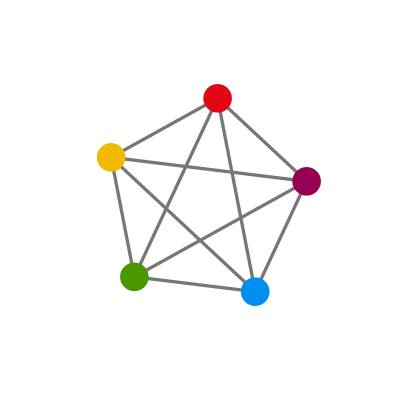
\includegraphics[scale=0.5]{./ej3/completo.jpg}
 	{\\Gráfico 3.4.3 - Grafo completo}
  \end{center}
  \vspace*{0.3cm}
  
  \vspace*{0.3cm} \vspace*{0.3cm}
  \begin{center}
 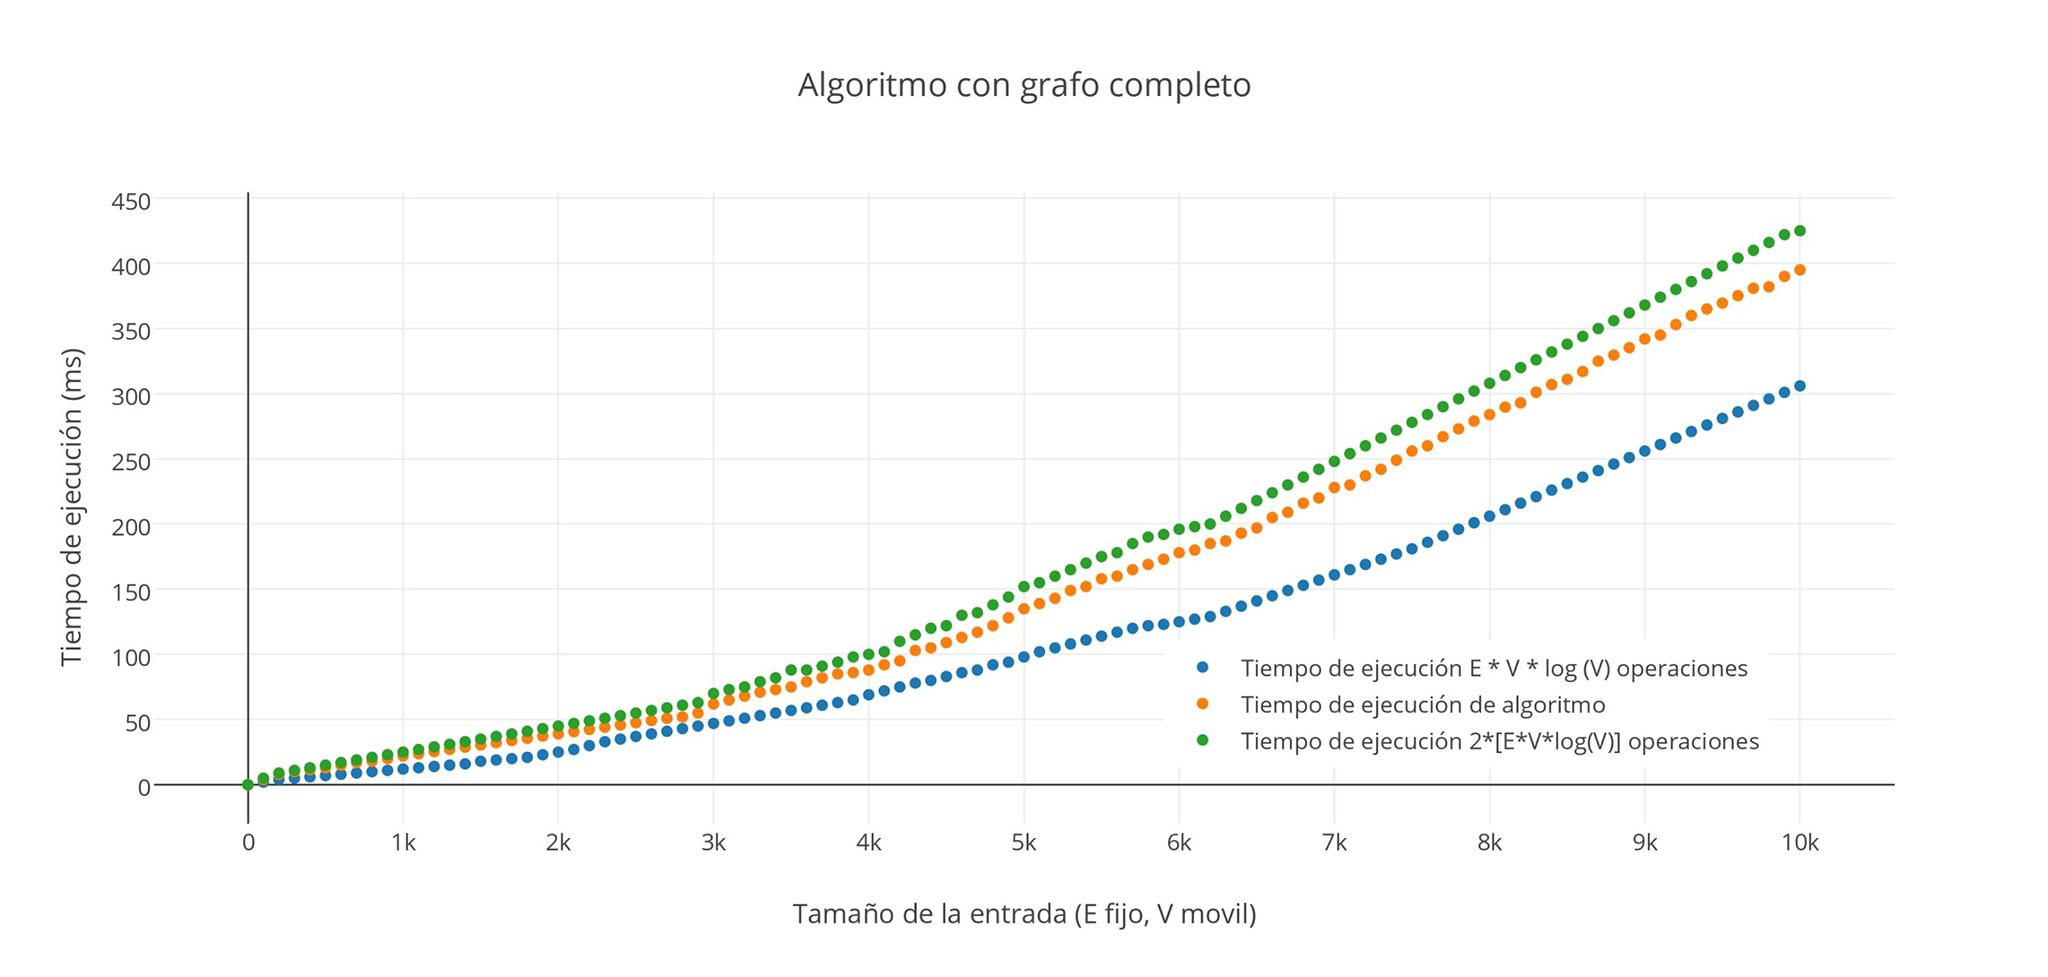
\includegraphics[scale=0.28]{./ej3/completo2.jpg}
 	{Gráfico 3.4.4 - Medición con grafo completo}
  \end{center}
  \vspace*{0.3cm}

En la figura 3.4.3 se puede observar el tipo de grafo que utilizamos. En la figura 3.4.4, se puede ver como el tiempo de ejecución de nuestro algoritmo es un poco mayor que un grafo circular, ya que tenemos más nodos interconectados y a pesar de esta situación nos mantenemos dentro de los tiempos estipulados corroborando la complejidad calculada.\\


Trabajando con grafos en el cual todos los nodos estan conectados unicamente con el del centro variando el tamaño de entrada entre 0 y 10000 y corriendo la misma medición varias veces sacamos un promedio del mismo para obtener datos  más relevantes y obtuvimos el siguiente resultado:

\vspace*{0.3cm} \vspace*{0.3cm}
  \begin{center}
 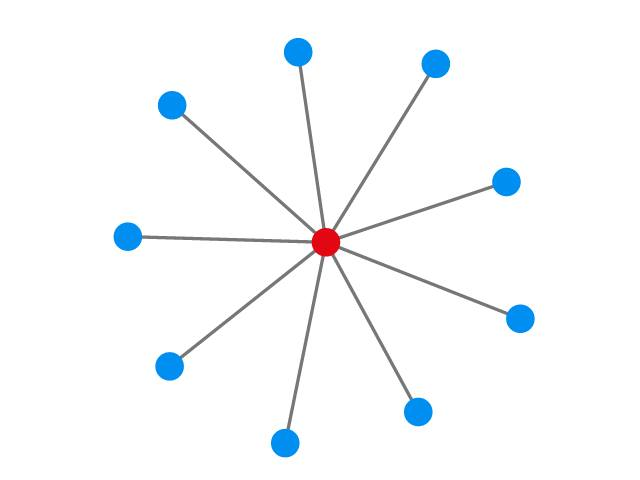
\includegraphics[scale=0.5]{./ej3/uniconodo.jpg}
 	{\\Gráfico 3.4.5 - Grafo único nodo conectado con todos}
  \end{center}
  \vspace*{0.3cm}
  
  \vspace*{0.3cm} \vspace*{0.3cm}
  \begin{center}
 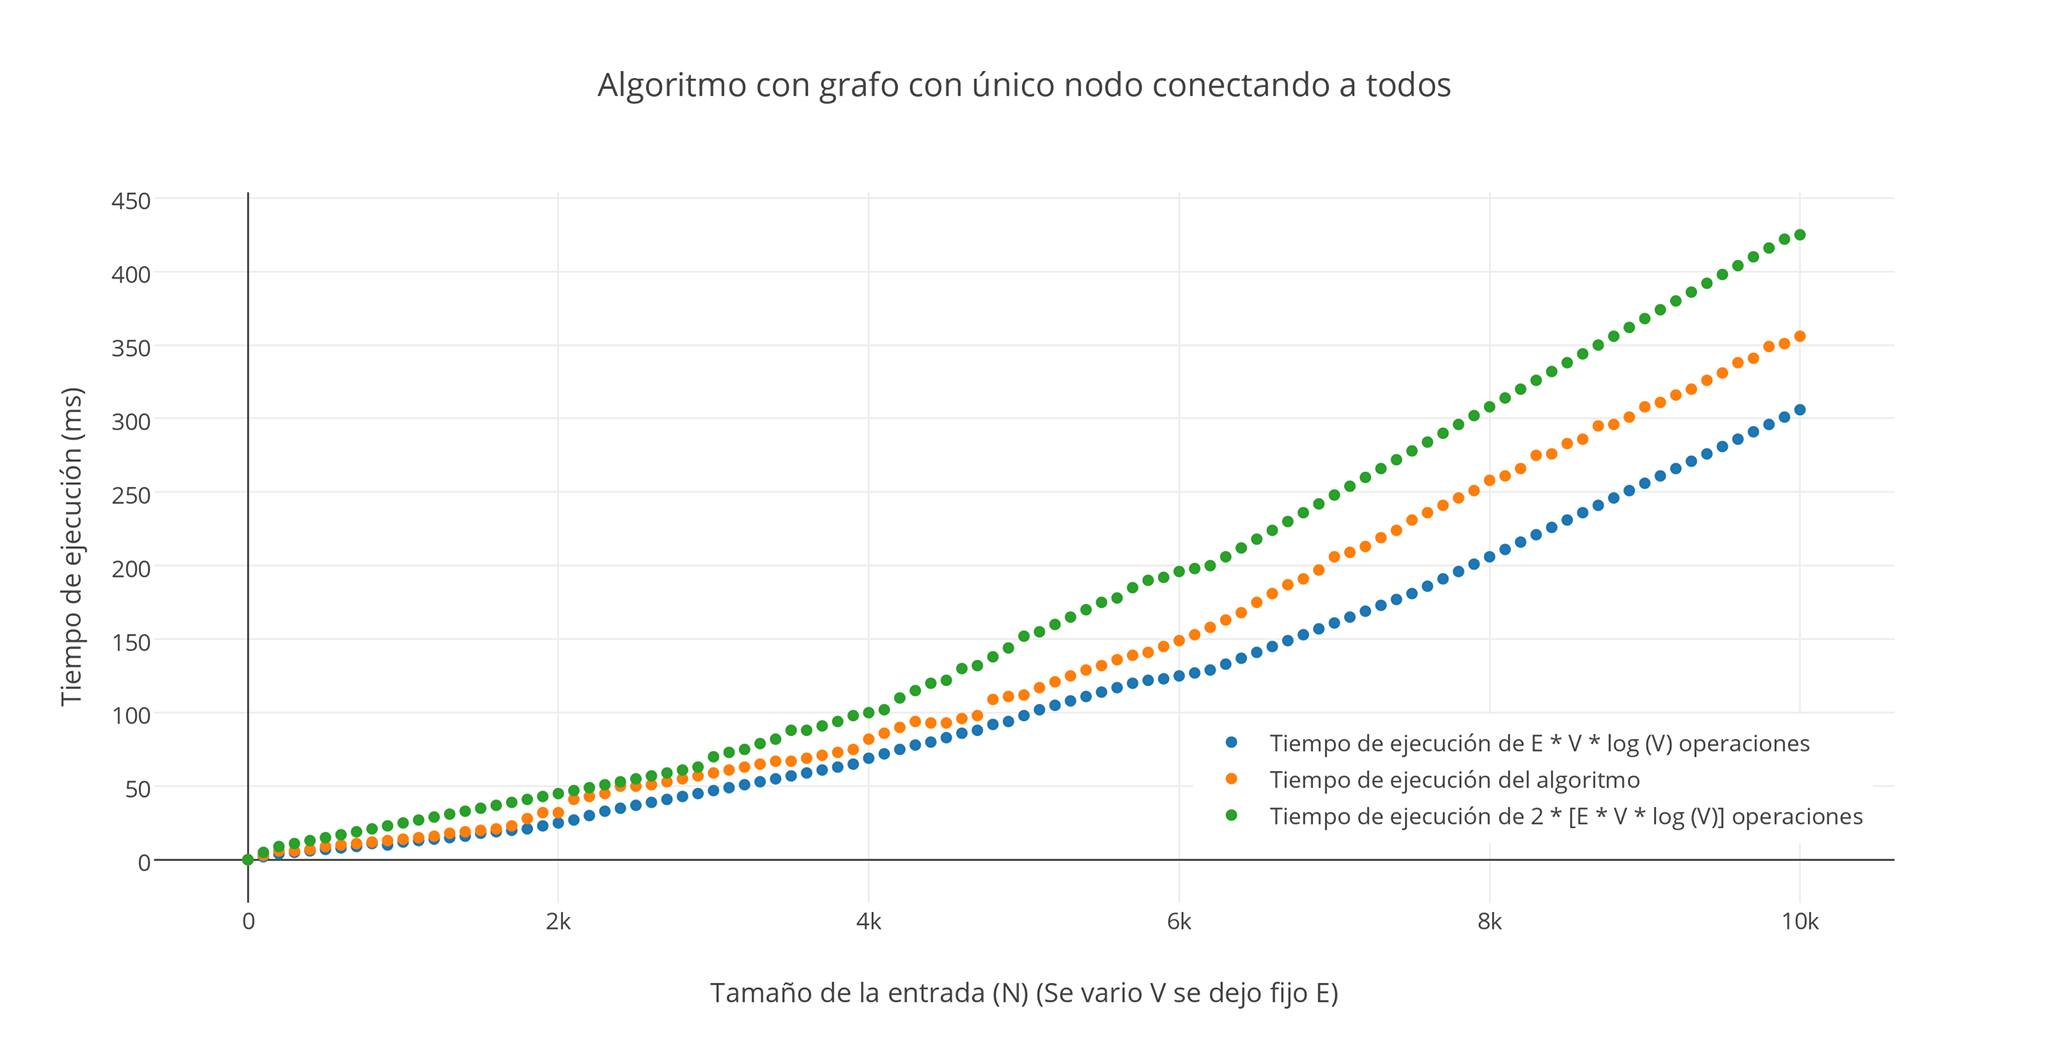
\includegraphics[scale=0.28]{./ej3/uniconodo2.jpg}
 	{Gráfico 3.4.6 - Medición Grafo único nodo conectado con todos}
  \end{center}
  \vspace*{0.3cm}

En la figura 3.4.5 se puede observar el tipo de grafo que utilizamos. En la figura 3.4.6, se puede ver como el tiempo de ejecución de nuestro algoritmo es similar e inferior al grafo circular ya que un único nodo se encuentra conectados con todos\\

